\documentclass[conference]{IEEEtran}
\IEEEoverridecommandlockouts
% The preceding line is only needed to identify funding in the first footnote. If that is unneeded, please comment it out.
%Template version as of 6/27/2024

\usepackage{cite}
\usepackage{amsmath,amssymb,amsfonts}
\usepackage{algorithmic}
\usepackage{graphicx}
\usepackage{textcomp}
\usepackage{xcolor}
\usepackage{multirow}
\def\BibTeX{{\rm B\kern-.05em{\sc i\kern-.025em b}\kern-.08em
    T\kern-.1667em\lower.7ex\hbox{E}\kern-.125emX}}
\begin{document}

\title{Entropy-Gated Triplet Cross-Memory-Bank Learning for Long-Tailed Multi-Label Chest X-Ray Classification}

\author{
\IEEEauthorblockN{Dr. Christian Wagner}
\IEEEauthorblockA{\textit{Professor of Computer Science}\\
The University of Nottingham\\
Nottingham, United Kingdom\\
Christian.Wagner@nottingham.ac.uk}
\and
\IEEEauthorblockN{Dr. Shreyank Narayana Gowda}
\IEEEauthorblockA{\textit{Assistant Professor}\\
The University of Nottingham\\
Nottingham, United Kingdom\\
Shreyank.NarayanaGowda@nottingham.ac.uk}
\and
\IEEEauthorblockN{Dr. Nguyen Trung Ky}
\IEEEauthorblockA{\textit{Professor of Computer Science}\\
International University - VNU\\
Ho Chi Minh City, Viet Nam\\
ntky@hcmiu.edu.vn}
\and
\IEEEauthorblockN{Ned Pham}
\IEEEauthorblockA{\textit{Student}\\
The University of Nottingham\\
Nottingham, United Kingdom\\
thien.pham@nottingham.ac.uk}
\and
\IEEEauthorblockN{Huy Pham}
\IEEEauthorblockA{\textit{Student}\\
International University - VNU\\
Ho Chi Minh City, Viet Nam\\
ititiu20216@student.hcmiu.edu.vn}
}

\maketitle

\begin{abstract}
In this paper, we propose a novel framework based on our submission to the ISBI 2026 CXR-LT Task~1 challenge \cite{b12} to enhance the performance of mAP for long-tailed, multi-label chest X-ray classification. In fact, with a two-stage ConvNeXt framework --- an ML-Decoder backbone trained with Asymmetric Loss
%~\cite{b3}
, then a sparse Mixture-of-Experts (MoE) decoder fine-tuning stage --- reaching an mAP of 0.4599 and third place 
%~\cite{b12}
, yet two problems central to that task stayed open: the aggregate mAP never showed whether rare (tail) findings, whose small positive gradient is dominated by the common findings they co-occur with, actually improve; and the MoE stage works against label co-occurrence itself, since per-token top-$k$ routing sends the tokens of a multi-finding study to different experts while the load-balancing loss that prevents expert collapse discourages any expert from specialising in findings that always appear together, so co-occurring labels receive fragmented, contradictory updates --- at a standing cost of expert and router parameters at inference. In this work, we keep the Stage-1 backbone and replace the MoE stage with a novel strategy including training-only regularizer of a \emph{single shared} embedding space, namely an entropy-gated triplet objective over a cross-batch memory bank, whose anchors are chosen by predictive entropy so the metric-learning signal falls on the least-resolved --- predominantly rare and co-occurring --- samples to improve the batch triplet loss cross-memory bank, and whose bank supplies the same- and different-finding neighbours a mini-batch of eight cannot hold for a tail class. Added to Asymmetric Loss for a single fine-tuning epoch and discarded at inference, the stage matches the MoE Stage~2 on mAP and mAUC over five random seeds at no inference-time cost; we report head-, medium- and tail-class mAP to locate the gain, disclose a small calibration (mECE) regression, and find the effect replicates from a less converged Stage-1 checkpoint at a magnitude that tracks Stage-1 maturity.
\end{abstract}

\begin{IEEEkeywords}
Medical Image Classification, Long-Tail Distribution, Label Co-occurrence, Deep Metric Learning, Triplet Loss, Cross-Batch Memory, Entropy Sampling, ConvNeXt.
\end{IEEEkeywords}

\section{Introduction}
Automated multi-label classification of chest X-rays is complicated by two coupled statistical properties of clinical data: a long-tailed distribution of findings, in which a handful of common conditions account for the majority of positive labels while dozens of clinically important findings appear rarely, and pervasive label co-occurrence, in which rare findings are seldom observed in isolation. Together these effects make it difficult for a classifier to learn discriminative, class-specific representations for tail classes, since their gradient signal is small in absolute terms and is frequently entangled with that of co-occurring head classes.

In our submission to the ISBI 2026 CXR-LT Task~1 challenge~\cite{b12}, we addressed this problem with a two-stage ConvNeXt~\cite{b1} framework: a Stage-1 backbone trained end-to-end with an ML-Decoder~\cite{b2} classification head and Asymmetric Loss~\cite{b3}, followed by a Stage-2 fine-tuning phase that converted the top two ConvNeXt stages and the decoder's feed-forward layers into a sparse Mixture-of-Experts (MoE), trained with an auxiliary load-balancing loss. That framework obtained an mAP of 0.4599 on the official test set and secured third place in the competition.

While effective, the MoE stage leaves two questions open. First, a long-tailed benchmark is not won on the average, and the single aggregate mAP we reported does not reveal whether the MoE stage improved the rare findings it was partly designed for or merely sharpened the already-strong head classes. Second, the MoE stage sits awkwardly with the co-occurrence structure it is meant to model: sparse top-$k$ routing is applied per token, so the feature and per-class query tokens of a study containing several findings are dispatched to different experts, while the load-balancing loss that keeps every expert in use rewards spreading tokens uniformly and thus discourages the one behaviour --- a single expert consistently handling a recurring pair of findings --- that would let the model represent that co-occurrence jointly. The co-occurring findings are then refined through partly disjoint parameters whose gradients can pull the shared backbone in competing directions. These effects, together with the expert and router parameters that persist at inference and the extra fine-tuning epochs spent guarding against expert collapse, motivate a different question: can the same goal --- more discriminative representations for entangled tail findings --- be met by regularizing a \emph{single shared} embedding space during fine-tuning, rather than partitioning it? In this paper we pursue that route, leaving the Stage-1 architecture, and hence the deployed model, completely unchanged.

We propose an \emph{entropy-gated triplet cross-memory-bank} fine-tuning stage. A first-in-first-out memory bank accumulates pooled decoder embeddings and their multi-hot labels across many mini-batches, giving access to a much larger and more diverse pool of same-class and different-class examples than a mini-batch of size 8 could offer on its own. Rather than mining a triplet for every sample in the batch, we use the model's own predictive uncertainty as a filter: only the sample with the highest Shannon entropy over its predicted class distribution is used as an anchor at each step. The intuition is that low-entropy predictions are already confidently (and usually correctly) classified, so the metric-learning signal is spent most productively on the sample the current model is least sure about. For each selected anchor, the hardest positive (closest same-class embedding by label overlap) and hardest negative (farthest different-class embedding) are retrieved from the memory bank, and a standard margin-based triplet loss is added to the Asymmetric Loss classification objective.

Our contributions are as follows.
\begin{itemize}
\item We introduce an entropy-gated anchor selection rule for triplet mining that requires no additional trainable parameters and adds negligible compute, since the entropy of the classification logits is available for free at every training step.
\item We combine this with a cross-batch memory bank in the style of XBM~\cite{b6}, adapted to a multi-label setting through a label-overlap-based positive/negative definition.
\item We show, across five random seeds, that a single epoch of this fine-tuning stage improves mAP, mF1 and mAUC over its Stage-1 initialization --- with a small calibration (mECE) regression that we report rather than obscure --- and reaches mAP and mAUC comparable to our previously published MoE-based Stage~2, while leaving the deployed model architecture unchanged. We further break the improvement down by class frequency to show where it falls.
\item We report an empirical limitation of the approach: under our label-overlap criterion, only a small fraction of optimization steps yield a usable triplet, and we discuss what this implies for future work.
\end{itemize}

\section{Related Work}
\textbf{Long-tailed multi-label chest X-ray classification.} The CXR-LT 2026 challenge~\cite{b12} builds on PadChest~\cite{b9} and PadChest-GR~\cite{b10} to curate a 30-class long-tailed multi-label benchmark. Prior CXR-LT submissions, including our own~\cite{b12}, have generally combined a large pretrained backbone with reweighted or focal-style classification losses such as Asymmetric Loss~\cite{b3} to counteract the extreme negative/positive imbalance inherent to multi-label prediction.

\textbf{Query-based decoding heads.} Rather than pooling backbone features with global average pooling, several architectures decode one query embedding per class through cross-attention over the visual feature map, following the general recipe of DETR~\cite{b13}. ML-Decoder~\cite{b2}, used in our Stage-1 backbone, is one such scalable classification head; it is closely related to Query2Label, which we used to motivate the decoder design in our original submission~\cite{b12}.

\textbf{Deep metric learning and hard example mining.} Triplet losses were popularized for embedding learning by FaceNet~\cite{b4}, and subsequent work showed that mining the hardest positive and negative within a batch, rather than sampling triplets uniformly at random, is critical to convergence and final embedding quality~\cite{b5}. Because a mini-batch is a very small and noisy sample of the full hardness distribution, Cross-Batch Memory (XBM)~\cite{b6} proposed maintaining a memory bank of recent embeddings, which we adapt here to a multi-label setting.

\textbf{Entropy-based sample selection.} Predictive Shannon entropy is a standard uncertainty measure in active learning, where it is used to select the unlabeled examples most worth annotating~\cite{b7}. We repurpose this idea for a fully supervised setting: rather than selecting which examples to label, we use entropy to select which already-labeled examples are most worth using as anchors for metric-learning at the current point in training.

\textbf{Mixture-of-Experts fine-tuning.} Our prior Stage-2 approach followed the GShard~\cite{b8} sparse-routing design to introduce conditional computation into the top ConvNeXt stages and decoder feed-forward layers. The method proposed in this paper is intended as a lighter-weight alternative to that stage, not a replacement for the Stage-1 backbone itself.

\section{Proposed Method}
\begin{figure}[htbp]
\centerline{\includegraphics[width=\linewidth,page=5]{Entropy.pdf}}
\caption{Overview of the proposed Stage-2 fine-tuning pipeline. The Stage-1 ConvNeXt backbone and decoder are initialized from the frozen-free Stage-1 checkpoint and continue training with a Triplet Cross-Memory-Bank objective gated by Anchor-Based Entropy Selection, in place of the Mixture-of-Experts decoder used in our prior submission~\cite{b12}.}
\label{fig}
\end{figure}

\subsection{Overview}
As shown in Fig.~\ref{fig}, we retain the Stage-1 backbone from our prior work unchanged: a five-stage ConvNeXt encoder followed by an ML-Decoder~\cite{b2} head with $N{=}30$ learnable query embeddings, one per target label, and a two-dimensional positional encoding added to the backbone feature map before cross-attention, following DETR~\cite{b13}. Given an input image $x$, the backbone produces per-query decoder embeddings, which we mean-pool over queries and $\ell_2$-normalize into a single embedding $e \in \mathbb{R}^{768}$, and classification logits $y \in \mathbb{R}^{30}$. The Stage-1 checkpoint is trained end-to-end with Asymmetric Loss~\cite{b3} only; the contribution of this paper is entirely in how Stage 2 is fine-tuned from that checkpoint.

\subsection{Cross-Batch Memory Bank}
Given a mini-batch size of 8, the number of usable positive and negative pairs available for metric learning within a single batch is small, and the hardest examples encountered in a batch are a poor approximation of the hardest examples in the dataset as a whole. Following the spirit of XBM~\cite{b6}, we maintain a fixed-size memory bank $\mathcal{M}$ of $|\mathcal{M}|{=}96$ slots, implemented as a first-in-first-out ring buffer over embeddings and their corresponding multi-hot label vectors. After every optimization step, the current batch's embeddings and labels overwrite the oldest entries in the bank. Because the bank persists across steps, it exposes each anchor to a pool of embeddings up to $12\times$ larger than the mini-batch, drawn from many recent, slowly-drifting versions of the encoder.

\begin{figure}[htbp]
\centerline{\includegraphics[width=\linewidth,page=6]{Entropy.pdf}}
\caption{Triplet Cross-Memory-Bank pipeline: for each anchor embedding $e_i$ from the current mini-batch, pairwise distances to the memory bank $\mathcal{M}$ are computed, and the hardest positive (minimum distance among same-label memory entries) and hardest negative (maximum distance among different-label memory entries) are retrieved to form the triplet used in $\mathcal{L}_{tri}$ (Eq.~\ref{eq:triplet}).}
\label{fig:xbm}
\end{figure}

\subsection{Anchor-Based Entropy Selection}
Rather than mining a triplet for every sample in the batch, we select anchors using the model's own predictive uncertainty, illustrated in Fig.~\ref{fig:entropy}. For each sample $x_i$ in a batch $\mathcal{B}$, we compute the Shannon entropy of the softmax distribution over its classification logits,
\begin{equation}
H(x_i) = -\sum_{c=1}^{C} p_\theta(y_c \mid x_i)\,\log p_\theta(y_c \mid x_i),
\label{eq:entropy}
\end{equation}
and select as anchors the samples attaining the maximum entropy in the batch,
\begin{equation}
\mathcal{A} = \bigl\{\, x_i \in \mathcal{B} \;:\; H(x_i) = \max_{x_j \in \mathcal{B}} H(x_j) \,\bigr\}.
\label{eq:anchor}
\end{equation}
With a batch size of 8, $\mathcal{A}$ typically contains a single sample per step. The rationale is that a low-entropy prediction is one the current model is already confident about, and is therefore less informative to push around in embedding space; concentrating the (comparatively expensive) hard-mining and triplet computation on the single most uncertain sample per step directs the metric-learning signal toward the region of input space where the classifier's decision boundary is currently least well resolved.

\begin{figure}[htbp]
\centerline{\includegraphics[width=\linewidth,page=7]{Entropy.pdf}}
\caption{Anchor-Based Entropy Selection: the classification logits of every sample in the mini-batch are converted to a Shannon entropy score (Eq.~\ref{eq:entropy}), and the sample of maximum entropy is selected as the triplet anchor (Eq.~\ref{eq:anchor}).}
\label{fig:entropy}
\end{figure}

\subsection{Hard Positive/Negative Mining}
For each anchor $x_i \in \mathcal{A}$ with embedding $e_i$ and multi-hot label vector $\mathbf{y}_i$, we search the memory bank for a positive and a negative example. Because labels are multi-hot rather than mutually exclusive, we define positives as memory entries sharing \emph{more than one} label with the anchor, and negatives as memory entries sharing \emph{no} label with the anchor:
\begin{equation}
\mathcal{P}(i) = \{\, m \in \mathcal{M} : \mathbf{y}_m \cdot \mathbf{y}_i > 1 \,\},
\label{eq:posmask}
\end{equation}
\begin{equation}
\mathcal{N}(i) = \{\, m \in \mathcal{M} : \mathbf{y}_m \cdot \mathbf{y}_i = 0 \,\}.
\label{eq:negmask}
\end{equation}
The stricter, co-occurrence-aware threshold on $\mathcal{P}(i)$ avoids treating two samples that merely share the dominant, high-frequency ``Normal'' label as positives of one another. Within these sets, we mine the hardest pair by Euclidean distance in embedding space,
\begin{equation}
e_i^{+} = \operatornamewithlimits{arg\,min}_{m \in \mathcal{P}(i)} \lVert e_i - e_m \rVert_2, \qquad
e_i^{-} = \operatornamewithlimits{arg\,max}_{m \in \mathcal{N}(i)} \lVert e_i - e_m \rVert_2.
\label{eq:hardmine}
\end{equation}
If either $\mathcal{P}(i)$ or $\mathcal{N}(i)$ is empty, the anchor is skipped for that step; we quantify how often this occurs in Section~\ref{sec:results}.

\subsection{Training Objective}
The mined triplets contribute a standard margin-based triplet loss,
\begin{equation}
\mathcal{L}_{tri} = \frac{1}{|\mathcal{A}'|}\sum_{i \in \mathcal{A}'} \max\bigl(0,\ \lVert e_i - e_i^{+}\rVert_2 - \lVert e_i - e_i^{-}\rVert_2 + \alpha \bigr),
\label{eq:triplet}
\end{equation}
where $\mathcal{A}'\subseteq\mathcal{A}$ is the subset of anchors for which a valid positive and negative were found, and $\alpha{=}0.5$ is the triplet margin. When $\mathcal{A}'$ is empty, $\mathcal{L}_{tri}$ is treated as zero for that step. The full training objective combines this with the Asymmetric Loss classification term,
\begin{equation}
\mathcal{L} = \mathcal{L}_{ASL} + \lambda_{tri}\,\mathcal{L}_{tri},
\label{eq:total}
\end{equation}
with $\lambda_{tri}{=}0.1$. Following the class-frequency reweighting used in our prior submission, $\mathcal{L}_{ASL}$ uses focusing parameters $\gamma_{neg}{=}2.0$, $\gamma_{pos}{=}0.0$, probability shift (clip) $0.05$, and per-class weights on the positive term computed from inverse log class frequency and clipped to $[0.5, 2.0]$, so that rare classes contribute a somewhat larger positive gradient without destabilizing training on the most frequent classes.

\section{Experimental Setup}
We initialize from a Stage-1 checkpoint trained with the same ConvNeXt/ML-Decoder architecture and Asymmetric Loss objective as our prior submission~\cite{b12}, using an internal train/validation split drawn from the CXR-LT 2026 Task~1 training data with 30 target labels. Stage-2 fine-tuning uses AdamW with a learning rate of $3\times10^{-5}$, weight decay $0.01$, a cosine learning-rate schedule, batch size 8 with gradient accumulation over 6 steps (effective batch size 48), and mixed-precision training. Images are resized to $512\times512$. Fine-tuning is run for a single epoch with early stopping (patience 1) monitored on validation mAP, matching the lightweight, single-pass nature of the proposed regularizer.

To isolate model-level stochasticity (weight initialization of newly added heads and dataloader shuffle order) from data-level stochasticity, we fix per-sample augmentation deterministically as a function of the sample key and epoch, independent of the training seed, and repeat Stage-2 fine-tuning under five seeds: 86, 123, 456, 789, and 1024. All five runs share the same Stage-1 initialization, memory bank size, and hyperparameters described above, and were executed as independent Slurm jobs across a mix of NVIDIA A6000 (48GB) and Ada 4500 (24GB) GPUs.

\section{Results and Discussion}
\label{sec:results}

\begin{table}[htbp]
\caption{Internal validation performance, all three rows sharing the same Stage-1 checkpoint used in our original submission~\cite{b12}. Stage-2 (proposed) is reported as mean $\pm$ sample standard deviation over 5 seeds.}
\begin{center}
\resizebox{\linewidth}{!}{%
\begin{tabular}{|l|c|c|c|c|}
\hline
\textbf{Method} & \textbf{mAP} & \textbf{mF1} & \textbf{mAUC} & \textbf{mECE} \\
\hline
Stage 1 (backbone)~\cite{b12} & 0.385 & 0.395 & 0.875 & 0.134 \\
\hline
Stage 2: MoE~\cite{b12} & 0.405 & 0.402 & 0.882 & 0.130 \\
\hline
Stage 2: Proposed & \textbf{0.414} & \textbf{0.407} & \textbf{0.889} & 0.143 \\
 & $\pm$0.002 & $\pm$0.010 & $\pm$0.002 & $\pm$0.008 \\
\hline
\end{tabular}%
}
\label{tab1}
\end{center}
\end{table}

Table~\ref{tab1} reports internal validation performance, with all three rows measured from the identical Stage-1 checkpoint, giving a fully controlled comparison. Relative to its Stage-1 initialization, the proposed entropy-gated triplet cross-memory-bank stage improves mAP by 0.029, mF1 by 0.012, and mAUC by 0.014, all after only a single fine-tuning epoch. Calibration is not improved: mECE rises from 0.134 to 0.143, a modest but consistent regression that we discuss further below. The standard deviation across five seeds is small for mAP and mAUC (0.002) and moderate for mF1 (0.010), suggesting the discriminative gains are reliable rather than an artifact of a favorable seed.

Compared against the previously published MoE-based Stage 2~\cite{b12}, which was fine-tuned from the same Stage-1 checkpoint for two epochs, the proposed method reaches higher mAP (+0.009) and mAUC (+0.007) with comparable mF1 (+0.005) after only a single epoch of fine-tuning, while its calibration is modestly worse (mECE +0.013 relative to MoE). Unlike the MoE stage, the proposed method adds no expert or router parameters and requires no changes to the deployed model: the memory bank and triplet head are used only during training and are discarded entirely at inference time. The calibration regression observed for both Stage-2 variants relative to Stage 1 suggests it may be a general side effect of this fine-tuning step rather than something specific to either method, though confirming that would require calibrating a wider set of fine-tuning objectives, which we leave to future work.

\subsection{Sensitivity to Stage-1 Checkpoint Maturity}
The result above depends on the quality of the Stage-1 checkpoint being extended. To test this, we repeated the identical Stage-2 fine-tuning recipe and five-seed protocol from an independently trained Stage-1 checkpoint that had not yet converged (best validation mAP 0.377 after 7 epochs, versus 0.385 for the checkpoint used in Table~\ref{tab1}). Table~\ref{tab2} reports both pairs side by side.

\begin{table}[htbp]
\caption{Stage-2 (proposed) applied to two independently trained Stage-1 checkpoints of different maturity. Stage-2 rows are mean $\pm$ sample standard deviation over the same 5 seeds used in Table~\ref{tab1}.}
\begin{center}
\resizebox{\linewidth}{!}{%
\begin{tabular}{|l|l|c|c|c|c|}
\hline
\textbf{Checkpoint} & \textbf{Stage} & \textbf{mAP} & \textbf{mF1} & \textbf{mAUC} & \textbf{mECE} \\
\hline
\multirow{2}{*}{Converged~\cite{b12}} & 1 & 0.385 & 0.395 & 0.875 & 0.134 \\
\cline{2-6}
 & 2 (ours) & 0.414 & 0.407 & 0.889 & 0.143 \\
\hline
\multirow{2}{*}{Under-trained} & 1 & 0.377 & 0.376 & 0.879 & 0.148 \\
\cline{2-6}
 & 2 (ours) & 0.393 & 0.379 & 0.886 & 0.151 \\
\hline
\end{tabular}%
}
\label{tab2}
\end{center}
\end{table}

The under-trained checkpoint's own Stage-1 mAP (0.377) is close to, but not directly comparable with, the converged checkpoint's (0.385): mAUC is actually slightly higher for the under-trained checkpoint (0.879 vs.\ 0.875), while mAP, mF1 and mECE are all worse, consistent with a model that has learned a coarse decision boundary but has not yet sharpened per-class precision-recall trade-offs. Applying the proposed Stage 2 to this weaker checkpoint again improves mAP (+0.016), mF1 (+0.003) and mAUC (+0.007), the same direction as for the converged checkpoint, but with roughly half the absolute mAP gain (+0.016 vs.\ +0.029) and higher seed-to-seed variance in mF1 (std 0.014 vs.\ 0.010). Calibration again regresses slightly (mECE +0.003). We draw two conclusions from this experiment: first, the proposed method's benefit is not specific to one Stage-1 checkpoint and replicates in direction across an independently trained one; second, the size of that benefit and the achievable absolute mAP both scale with how well-converged the Stage-1 checkpoint already is, so Stage-1 training budget and Stage-2 fine-tuning are not fully independent design choices. At the time of writing, the under-trained checkpoint's own training job was still running, so the smaller gain reported here is a conservative, not necessarily final, estimate of the method's ceiling on that model lineage.

\subsection{Triplet Utilization Rate}
Because $\mathcal{P}(i)$ requires more than one shared label with the anchor and $\mathcal{N}(i)$ requires none, a step can easily fail to produce a usable triplet, particularly early in fine-tuning when memory bank entries with sufficient label overlap for the current anchor's rare classes may not yet be present. Across one full seed's training log, only 7.6\% of optimization steps produced a valid mined triplet; the remainder contributed only the Asymmetric Loss term for that step. This suggests that the effective learning rate of the triplet objective is considerably lower than $\lambda_{tri}{=}0.1$ would imply on its own, and that the gains reported in Table~\ref{tab1} are being driven by a comparatively small number of high-value updates. We view improving this utilization rate, for instance through a larger memory bank, a relaxed positive threshold for rare classes, or class-aware memory sampling, as the most direct avenue for future improvement.

\section{Conclusion}
We presented an entropy-gated triplet cross-memory-bank fine-tuning stage for long-tailed, multi-label chest X-ray classification, extending our prior two-stage ConvNeXt framework without altering its deployed architecture. By using the model's own predictive Shannon entropy to select which sample to use as a triplet anchor at each step, and mining hard positives and negatives from a persistent cross-batch memory bank, a single epoch of fine-tuning improves mAP, mF1, and mAUC over the Stage-1 backbone in a fully controlled, same-checkpoint comparison, and reaches mAP and mAUC comparable to our previously reported Mixture-of-Experts Stage~2 in a single epoch instead of two, at no additional inference-time cost; calibration is slightly worse than either the Stage-1 backbone or the MoE stage, which we report plainly rather than obscure. Repeating the full protocol on an independently trained, less mature Stage-1 checkpoint reproduces the same qualitative pattern at a smaller magnitude, showing that the gain is not specific to one checkpoint while also showing that it is sensitive to Stage-1 convergence. An empirical analysis further shows that only a small fraction of training steps currently yield a usable triplet under our multi-label positive/negative definition, which we identify, together with the calibration regression and the checkpoint-maturity dependence, as the primary limitations and directions for future work.

\section*{Acknowledgment}
The authors thank the organizers of the ISBI 2026 CXR-LT challenge for providing the benchmark dataset and evaluation infrastructure that made this comparison possible.

\begin{thebibliography}{00}
\bibitem{b1} Zhuang Liu, Hanzi Mao, Chao-Yuan Wu, Christoph Feichtenhofer, Trevor Darrell, and Saining Xie, ``A ConvNet for the 2020s,'' in IEEE/CVF Conference on Computer Vision and Pattern Recognition, CVPR 2022, New Orleans, LA, USA, June 18-24, 2022, pp. 11966--11976, IEEE.
\bibitem{b2} Tal Ridnik, Gilad Sharir, Avi Ben-Cohen, Emanuel Ben-Baruch, and Asaf Noy, ``ML-Decoder: Scalable and versatile classification head,'' arXiv:2111.12933, 2021.
\bibitem{b3} Tal Ridnik, Emanuel Ben Baruch, Nadav Zamir, Asaf Noy, Itamar Friedman, Matan Protter, and Lihi Zelnik-Manor, ``Asymmetric loss for multi-label classification,'' in 2021 IEEE/CVF International Conference on Computer Vision, ICCV 2021, Montreal, QC, Canada, October 10-17, 2021, pp. 82--91, IEEE.
\bibitem{b4} Florian Schroff, Dmitry Kalenichenko, and James Philbin, ``FaceNet: A unified embedding for face recognition and clustering,'' in IEEE Conference on Computer Vision and Pattern Recognition, CVPR 2015, Boston, MA, USA, June 7-12, 2015, pp. 815--823, IEEE.
\bibitem{b5} Alexander Hermans, Lucas Beyer, and Bastian Leibe, ``In defense of the triplet loss for person re-identification,'' arXiv:1703.07737, 2017.
\bibitem{b6} Xun Wang, Haozhi Zhang, Weilin Huang, and Matthew R. Scott, ``Cross-batch memory for embedding learning,'' in IEEE/CVF Conference on Computer Vision and Pattern Recognition, CVPR 2020, Seattle, WA, USA, June 13-19, 2020, IEEE.
\bibitem{b7} Burr Settles, ``Active learning literature survey,'' Computer Sciences Technical Report 1648, University of Wisconsin--Madison, 2009.
\bibitem{b8} Dmitry Lepikhin, HyoukJoong Lee, Yuanzhong Xu, Dehao Chen, Orhan Firat, Yanping Huang, Maxim Krikun, Noam Shazeer, and Zhifeng Chen, ``Gshard: Scaling giant models with conditional computation and automatic sharding,'' in 9th International Conference on Learning Representations, ICLR 2021, Virtual Event, Austria, May 3-7, 2021, OpenReview.net.
\bibitem{b9} Aurelia Bustos, Antonio Pertusa, Jose-Maria Salinas, and Maria de la Iglesia-Vaya, ``Padchest: A large chest x-ray image dataset with multi-label annotated reports,'' Medical Image Analysis, vol. 66, pp. 101797, 2020.
\bibitem{b10} Daniel Coelho de Castro, Aurelia Bustos, Shruthi Bannur, Stephanie L. Hyland, Kenza Bouzid, Maria Teodora Wetscherek, Maria Dolores S\'anchez-Valverde, Lara Jaques-P\'erez, Lourdes P\'erez-Rodr\'iguez, Kenji Takeda, Jos\'e Mar\'ia Salinas-Serrano, Javier Alvarez-Valle, Joaqu\'in Galant-Herrero, and Antonio Pertusa, ``Padchest-gr: A bilingual chest x-ray dataset for grounded radiology report generation,'' NEJM AI, vol. 2, no. 7, June 2025.
\bibitem{b11} Hexin Dong, Yi Lin, Pengyu Zhou, Fengnian Zhao, Alan Clint Legasto, Mingquan Lin, Hao Chen, Yuzhe Yang, George Shih, and Yifan Peng, ``Overview of the cxr-lt 2026 challenge: Multi-center long-tailed and zero shot chest x-ray classification,'' arXiv preprint arXiv:2602.22092, 2026.
\bibitem{b12} Huy Le Pham, Khoa Ha Anh, Nguyen-Thanh-Thao Vo, Ky Trung Nguyen, Chau Ly Thi Huyen, Hien Q. Ta, and Thang Doan Van, ``An efficient framework for long-tailed and multi-label classification on chest X-rays,'' ISBI 2026 Task 1, 2026.
\bibitem{b13} Nicolas Carion, Francisco Massa, Gabriel Synnaeve, Nicolas Usunier, Alexander Kirillov, and Sergey Zagoruyko, ``End-to-end object detection with transformers,'' in Computer Vision - ECCV 2020 - 16th European Conference, Glasgow, UK, August 23-28, 2020, Proceedings, Part I, vol. 12346 of Lecture Notes in Computer Science, pp. 213--229, Springer.
\end{thebibliography}

\end{document}
